\documentclass[10pt]{article}
\usepackage[a4paper,margin=2.2cm]{geometry}
\usepackage[T1]{fontenc}
\usepackage[utf8]{inputenc}
\usepackage{graphicx}
\usepackage{booktabs}
\usepackage{amsmath}
\usepackage{hyperref}
\usepackage{caption}
\usepackage{titlesec}
\usepackage{tikz}
\usetikzlibrary{positioning}
\captionsetup{font=small,labelfont=bf}
\setlength{\parskip}{2pt}
\titleformat{\section}{\large\bfseries}{\thesection}{0.6em}{}
\titleformat{\subsection}{\normalsize\bfseries}{\thesubsection}{0.5em}{}

% ---------------------------------------------------------------
% FRP 2026 -- ISSAI, Nazarbayev University
% Paste the sections below into the template's "Write here" boxes,
% or compile this file directly in Overleaf (upload images/ first).
% ---------------------------------------------------------------

\begin{document}

\begin{center}
{\LARGE\bfseries Can One Pipeline Turn a School Topic into a Finished Lesson Video in Three Languages?\par}
\vspace{4pt}
{\large A one-pipeline system for trilingual school lesson videos\par}
\vspace{8pt}
[Your Name]\quad [Teammate's Name]\\
Track: [Track Name]\\
ISSAI, Nazarbayev University\\
October 2026
\end{center}

\begin{abstract}
\noindent
Students need far more short learning material than teachers can produce by hand, especially in Kazakh, Russian and English. We built one pipeline in which a chat model writes a lesson script, an AI checker reads it, an image model draws each scene, a speech model narrates it, and ffmpeg renders a finished video with chapter marks, a quiz and a gallery card. The pipeline produced 75 videos covering 7 school subjects (82 minutes, 219 quiz questions) at about 3 minutes of build time per video, whereas the same video made by hand is estimated at 60--120 minutes. This matters because it lets one teacher equip a whole class with multilingual, quiz-ready material in the time a single hand-made video used to take.
\end{abstract}

\begin{figure}[t]
\centering
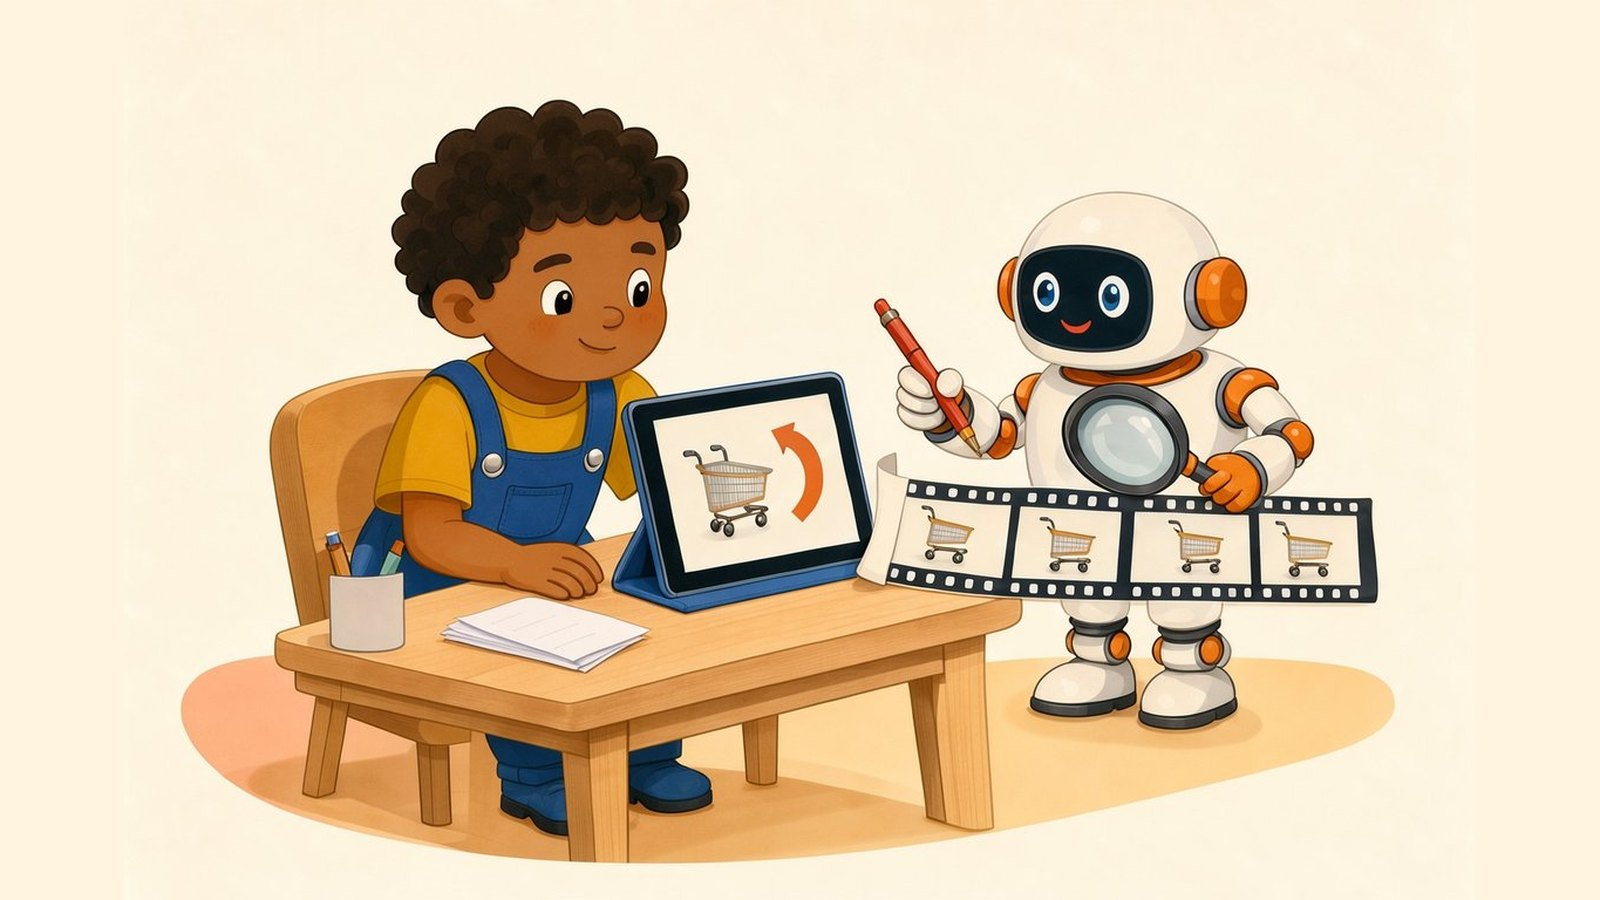
\includegraphics[width=\textwidth]{images/teaser.jpg}
\caption{A student watches a lesson at a laptop while a robot assembles the same topic into a filmstrip of generated scenes, illustrating the topic-to-video pipeline.}
\label{fig:teaser}
\end{figure}

\section{Introduction}

A teacher who wants a short video on, for example, ``Newton's second law'' for Grade 9 in Kazakh has to write a script, find pictures, record a voice and edit everything, and a student revising alone at night has no such video at all. In our own school experience, the topics asked for most often (physics, chemistry and history) are exactly the ones with the fewest ready-made clips in Kazakh or Russian.

What is missing today is not a video generator but an end-to-end school tool: large text-to-video models produce beautiful silent clips, yet they do not write a curriculum-correct script, do not add a narrated explanation in Kazakh or Russian, do not produce chapter marks or a quiz, and cannot be searched by subject and grade. Teachers also cannot easily correct a single wrong scene inside a generated clip.

We built a white-box pipeline around existing class models and rendered 75 curriculum videos with it, reaching about 3 minutes per finished video against an estimated 60--120 minutes by hand. Our contributions are: (1) a script-first pipeline that checks the text before any picture or voice is generated; (2) a trilingual gallery with subject, grade and language filters, chapter marks and quizzes; (3) a public release of 75 videos and the full measurement, with an honest report of what is still weak.

\section{Related Work}

Singer et al.~\cite{singer2022} train a diffusion model on text--image pairs to generate short silent video clips; their system is impressive but needs large video corpora, and the output cannot easily be edited scene by scene or narrated in Kazakh. Khachatryan et al.~\cite{khachatryan2023} obtain zero-shot video from a pretrained image diffusion model by moving the latent code; this removes training data but still yields silent motion clips without captions, chapters or quizzes. Brooks et al.~\cite{brooks2024} describe large-scale video generation models as world simulators, showing strong visual quality at a cost and scale that a school cannot run.

Our work differs in three ways: we do not train or run a video-generation model at all, we keep every intermediate artefact (script, one image per scene, audio, captions) editable, and we target a fixed school format -- 1--1.5 minutes, three languages, chapter marks, a quiz and a searchable card.

\section{What We Built}

\textbf{Input.} The user gives a topic, a school grade and a language (Kazakh, Russian or English) on the ``Create'' page, or uploads an existing video or a PDF lesson.

\textbf{AI.} A chat model from the DeepSeek family~\cite{deepseek2024} (DeepSeek-V4.1-Flash, served through the class API; the parameter count is not public) writes a scene-by-scene script with a title, narration and image prompts. A second AI check reads the script for factual and curriculum errors before anything else is generated. The image model FLUX.3 klein (Black Forest Labs) draws one picture per scene, and the OmniVoice speech model narrates each scene in the chosen language. We do not fine-tune any model: all models are used zero-shot through the class API.

\textbf{Output.} ffmpeg scales the pictures to 1080p, aligns each scene with its narration, adds burned-in captions and chapter marks, and encodes an MP4 in the project convention \texttt{out/<slug>-<lang>.mp4}; the gallery then shows a card with subject, grade and language tags, and the quiz page shows the questions before and after the video.

\textbf{Data and resources.} There is no training dataset: the 75 topics were written by us from the school curriculum across 7 subjects (biology, chemistry, geography, history, languages, mathematics, physics). Generated images and audio are produced by the class models; the code and metadata are public. Model calls ran on the ISSAI GPU server through the class API proxy, and rendering ran on the workspace CPU with ffmpeg.

\begin{figure}[t]
\centering
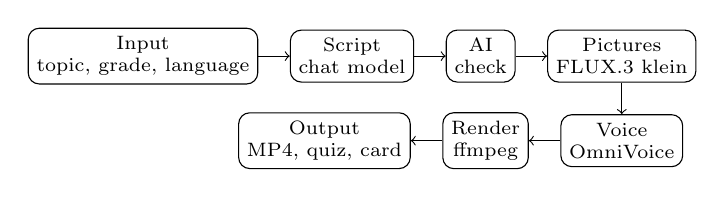
\begin{tikzpicture}[node distance=4mm,
  box/.style={draw, rounded corners, align=center, font=\scriptsize, inner sep=3pt}]
\node[box] (in) {Input\\topic, grade, language};
\node[box, right=of in] (sc) {Script\\chat model};
\node[box, right=of sc] (ch) {AI\\check};
\node[box, right=of ch] (im) {Pictures\\FLUX.3 klein};
\node[box, below=of im] (vo) {Voice\\OmniVoice};
\node[box, left=of vo] (rn) {Render\\ffmpeg};
\node[box, left=of rn] (out) {Output\\MP4, quiz, card};
\draw[->] (in) -- (sc);
\draw[->] (sc) -- (ch);
\draw[->] (ch) -- (im);
\draw[->] (im) -- (vo);
\draw[->] (vo) -- (rn);
\draw[->] (rn) -- (out);
\end{tikzpicture}
\caption{How it works: a topic and a language go in, four models write, draw, speak and render, and a searchable video with chapter marks and a quiz comes out.}
\label{fig:pipeline}
\end{figure}

\begin{figure}[t]
\centering
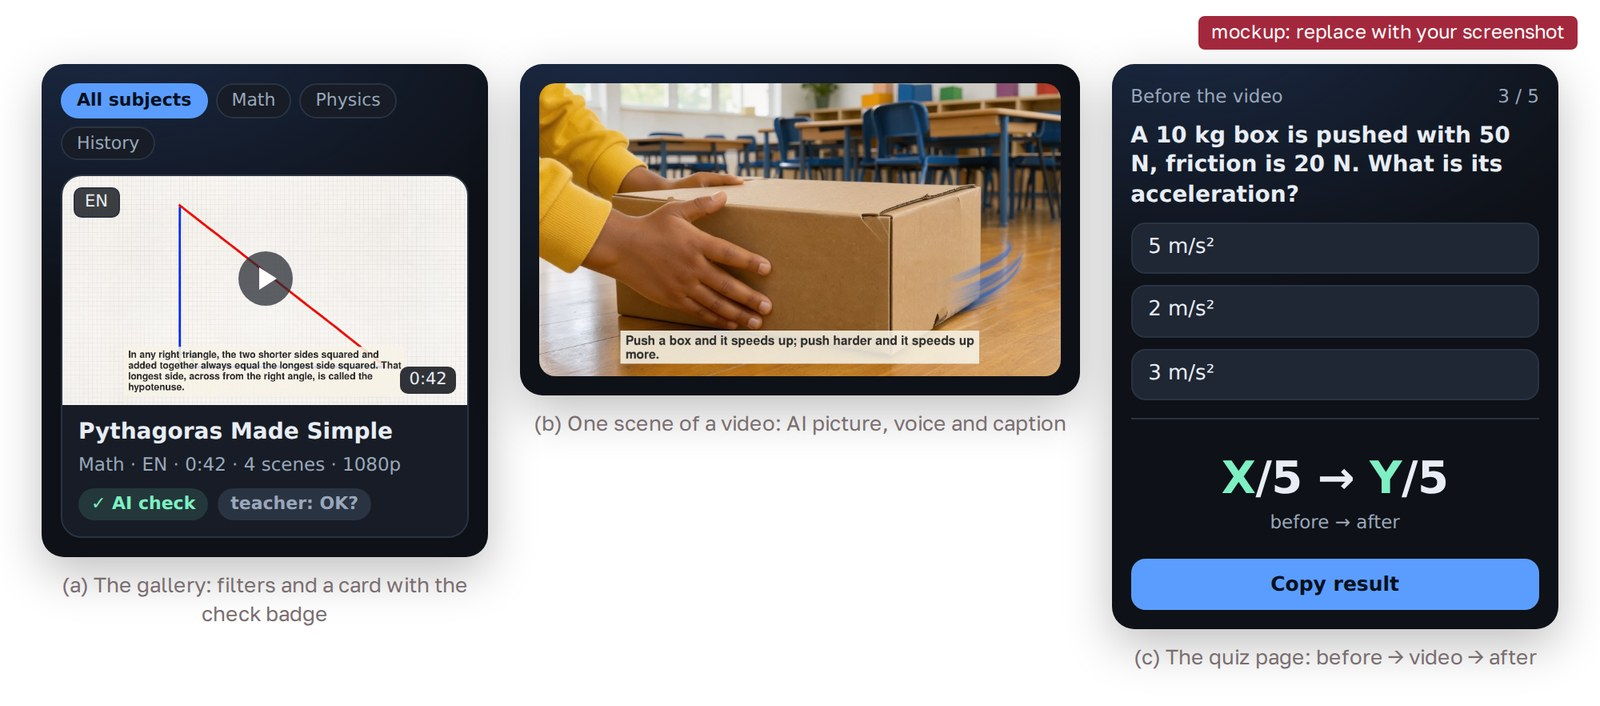
\includegraphics[width=\textwidth]{images/demo.jpg}
\caption{The three surfaces of the system: (a) the gallery with filters and a check badge, (b) one generated scene with its narration caption, and (c) the quiz page that shows the score before and after the video.}
\label{fig:demo}
\end{figure}

\section{How We Measure}

We count a video as \emph{correct} if it finishes rendering, its duration is between 45 and 120 seconds, every scene has a picture, narration and caption, and the script passes the automated check; a video is \emph{wrong} if it fails to render, has a missing scene or a factual error flagged by the checker. The baseline is the old way: one teacher making the same 1--1.5-minute video by hand (script, slides, voice recording, editing), which we estimate at 60--120 minutes per video; this baseline is an estimate and was not timed by us. Our measure is the build time recorded by the pipeline for each of the 75 videos on the same machine.

Our pipeline has no training stage, so the test topics are unseen by construction: each topic was fixed before generation and no prompt was tuned on the reported builds. All numbers below come from \texttt{data.json} and the build logs in the repository.

\section{Results}

\begin{table}[h]
\small
\centering
\caption{One hand-made video versus the pipeline, on the same school format (1--1.5 minutes, narrated, captioned). Time is per finished video; the arrow shows that lower is better.}
\label{tab:main}
\begin{tabular}{lccc}
\toprule
Approach & Videos & Total minutes & Time per video (min) $\downarrow$ \\
\midrule
Baseline: hand-made (estimated) & 1 & 1.1 & 60--120 \\
Ours: AI pipeline (measured)     & 75 & 82 & $\approx$3 \\
\bottomrule
\end{tabular}
\end{table}

Table~\ref{tab:main} shows that the pipeline produced 75 videos and 82 minutes of finished material, about 20--40 times faster per video than the estimated hand-made baseline. Coverage is broad rather than perfect: 73 of 75 videos carry a school grade and chapter marks, and the gallery offers 219 quiz questions across 7 subjects.

The quality evidence is narrower. Only 24 scripts were sent to the automated check (the checker was added after the first videos), of which 15 passed and 9 were stopped; the remaining 51 were never checked. All timing numbers come from a single machine and a single run per video, so the speed ratio is indicative rather than a controlled benchmark.

\section{Limitations}

The main boundary is quality control: two thirds of the gallery was built before the checker existed, so the ``checked'' badge covers only 15 videos, and the checker itself is an AI model that can miss factual errors. Pictures are generated at 1536 px and upscaled to 1080p, so they look soft on a large screen, and a wrong scene currently means rebuilding the whole video rather than editing one frame. The speed comparison uses an estimated baseline on one machine with no repeated runs, and no human evaluators scored the videos; Kazakh narration in particular has not been rated by native speakers. The next step is to run the checker on the remaining 51 scripts, regenerate pictures at higher resolution, and test the result with a class of students.

\section{Ethics}

All content is generated from curriculum topics written by us; no student data, private photos, voice recordings or personal information were used or published, and the gallery contains only generated pictures and synthetic narration. The models are accessed through the class API under the course's terms, the generated outputs are released with the project, and the code and metadata are public. We checked that no API keys, tokens or private files appear in the repository. We used an AI coding agent to write code and to check the English.

\section{Conclusion}

We built and measured a white-box pipeline that turns a school topic into a narrated, captioned, quiz-ready video in Kazakh, Russian or English, and released 75 such videos in a searchable gallery. The pipeline reached about 3 minutes per video against an estimated 60--120 minutes by hand, while the automated check passed 15 of 24 scripts and stopped 9. Next we will check the remaining scripts, raise picture resolution, and evaluate the videos with real students in class.

\section*{Acknowledgments}

We thank the FRP 2026 mentors and the ISSAI class API team. Project page: \url{https://basiggs.github.io/frp-2026/projects/diar-page/}. Code and data: \url{https://github.com/Basiggs/frp-2026}.

\begin{thebibliography}{9}

\bibitem{singer2022}
U.~Singer, A.~Polyak, T.~Hayes, X.~Yin, J.~An, S.~Zhang, Q.~Hu, H.~Yang, O.~Ashual, O.~Gafni, D.~Parikh, S.~Gupta, and Y.~Taigman.
\newblock Make-A-Video: Text-to-video generation without text-video data.
\newblock \emph{arXiv preprint arXiv:2209.14792}, 2022.

\bibitem{khachatryan2023}
L.~Khachatryan, A.~Movsisyan, V.~Tadevosyan, R.~Henschel, Z.~Wang, S.~Navasardyan, and H.~Shi.
\newblock Text2Video-Zero: Text-to-image diffusion models are zero-shot video generators.
\newblock In \emph{Proceedings of the IEEE/CVF International Conference on Computer Vision (ICCV)}, 2023.

\bibitem{brooks2024}
T.~Brooks, B.~Peebles, C.~Holmes, W.~DePue, Y.~Guo, L.~Jing, D.~Schnurr, J.~Taylor, T.~Luhman, E.~Luhman, C.~Ng, R.~Wang, and A.~Ramesh.
\newblock Video generation models as world simulators.
\newblock Technical report, OpenAI, 2024.

\bibitem{deepseek2024}
DeepSeek-AI.
\newblock DeepSeek-V3 technical report.
\newblock \emph{arXiv preprint arXiv:2412.19437}, 2024.

\end{thebibliography}

\end{document}
